\section{Introduction}
C language can be used in embedded design with Nios processor and SystemC. This tutorial contains various features of C language, which we will need for designing the SoPC (system on programmable chip) using NiosII processor. Further, the tutorials on `SoPC design using C/C++' can be found at the \href{http://pythondsp.readthedocs.io/en/latest/pythondsp/toc.html}{website} under the Section `VHDL/Verilog tutorials'.  In this chapter, simple `Hello World' program is discussed along with it's execution. 


%\section{What is program}
%\textbf{Program} is the collection of statements written in some language e.g. Python, C or VHDL etc. to perform certain operations. 
%\\ \\
%\textbf{Compiler} is required to convert the program to assembly language (machine language); which is used by assembler. 
%\\ \\
%\textbf{Assembler} converts the assembly language code to object code; which is used by linker. 
%\\ \\
%\textbf{Linker} links the various source codes referenced by the main-source-code and/or rum-time libraries, to generate the executable file which is used by loader. 
%\\ \\
%\textbf{Loader} executes the executable file to generate the outputs of the source codes. 

\section{Installing Compiler}
We only need a C compiler to execute the programs. There are various C/C++ compiler available on Internet. Some of the C/C++ compilers are discussed below, so that we can compile both C and C++ codes. 
\\ \\
\textbf{Linux:} To install the compiler on Linux, type following command to the terminal, \\
\textbf{\textdollar  { \ }  sudo apt-get install g++}
\\ \\
\textbf{Windows:} Install `mingw' compiler and add it to windows path; or `code:block software' which contains the mingw compiler and set the mingw in the path after installation. Other options are also available e.g. Borland C or Turbo C etc.

\section{Writing first code}
 Listing \ref{c:helloWorld} shows the source code to print the `Hello World' on the screen. To execute the code in the listing, open the terminal and go to the folder where program is saved and type following commands; which will generate the output on the terminal. 
\\
\textbf{\textdollar { \ } gcc helloWorld.c -o out} \\
\textbf{\textdollar { \ }  ./out} (in Unix)\\
\textbf{\textdollar { \ }  out} (in Windows)\\

\begin{explanation}[Listing \ref{c:helloWorld}]
	Note that, C is \textbf{case-sensitive} language. Each program contains one and only one  `main' function, which is the starting point of the code. In this listing, Line 6 has the `main' function, which contains two other keywords i.e. `int' and `void'; here `void' indicates that, the main `function' does not have any input parameter, whereas `int' represents that the return type of this function is `integer'. 
	
	\textbf{Keywords} are nothing but predefined words in C, which can not be used for declaring \textbf{Identifiers} i.e. name of variables, functions and array etc. Table \ref{tbl:KeywordsC} shows the list of keywords available in C and C++ languages. Further, the terms `function', `parameters' and `return type' are discussed in Chapter \ref{FunctionPointer}. Further, all the statements inside the brackets (\{ \}) (i.e. between Line 7 and 11) are belongs to function `main'. 
	
	\begin{table}
		\centering
		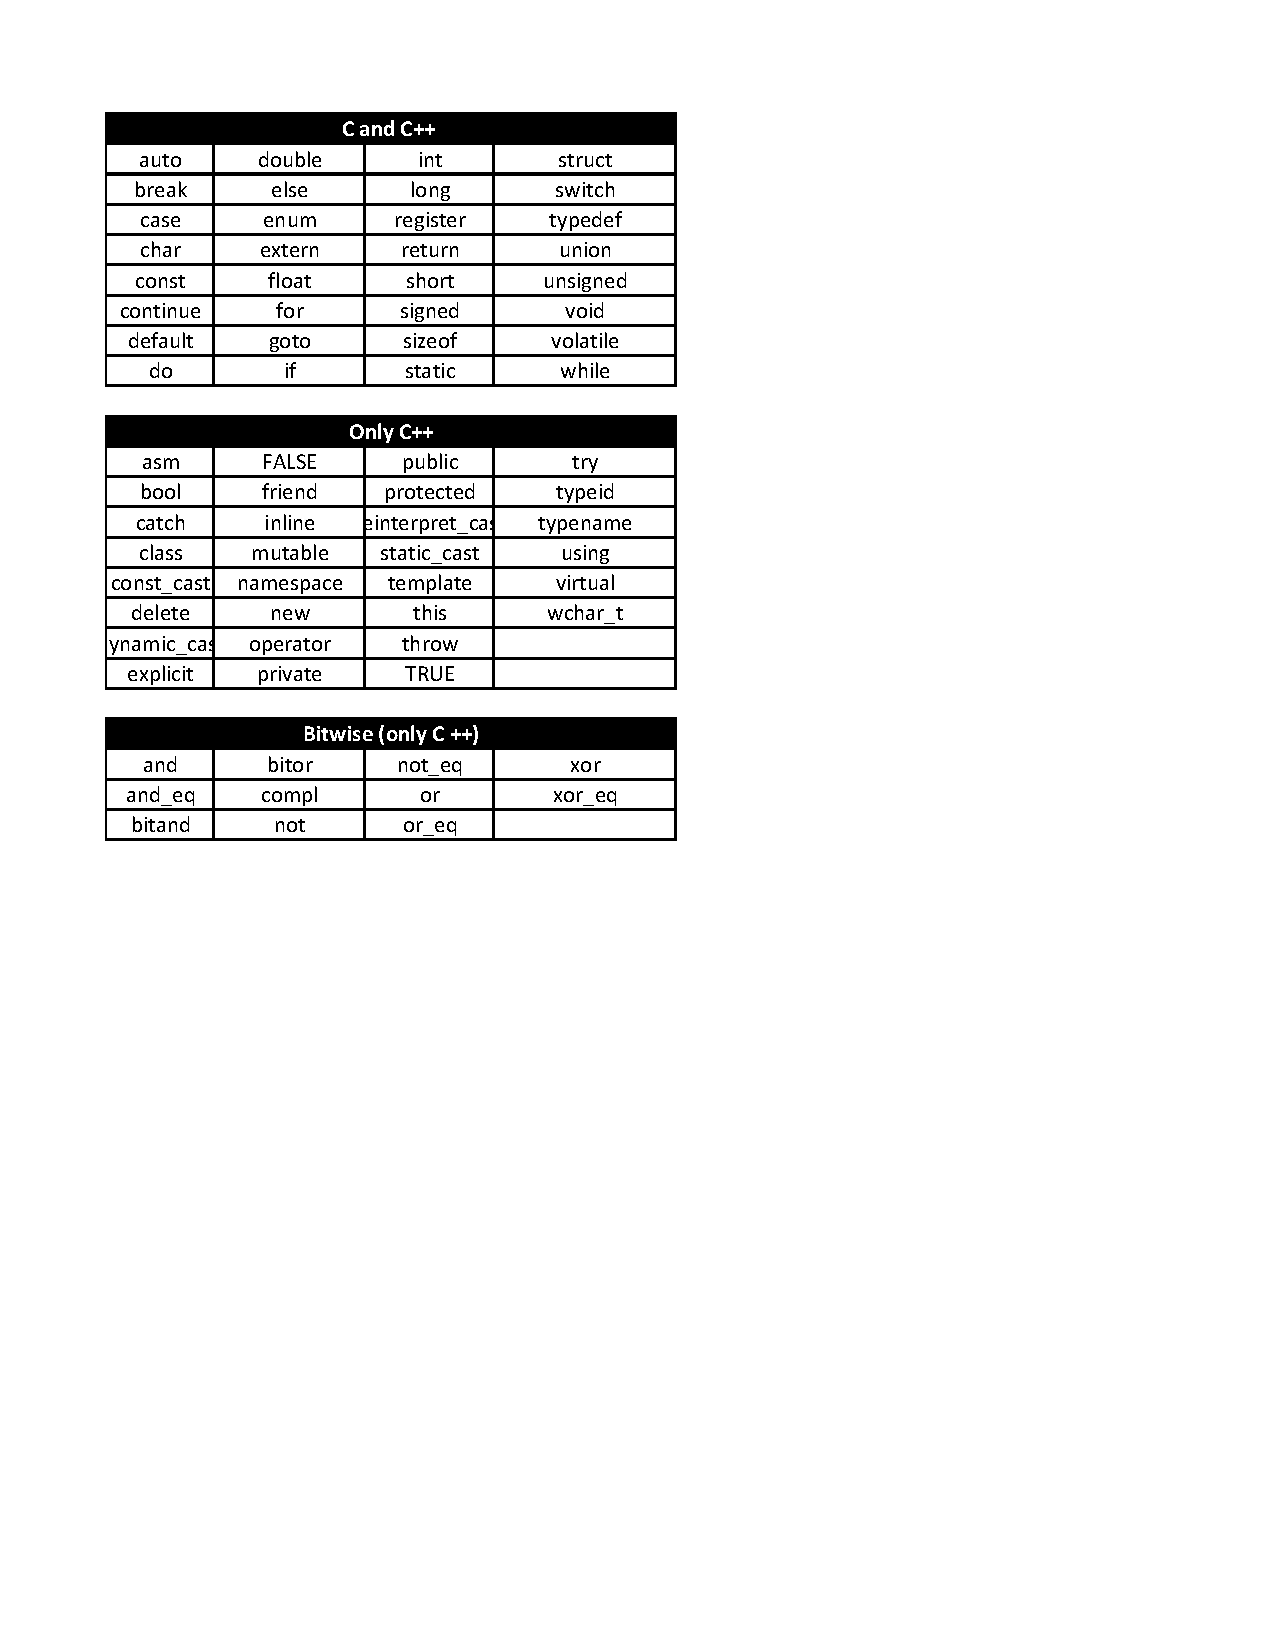
\includegraphics{KeywordsCpp}
		\caption{Keywords in C and C++}
		\label{tbl:KeywordsC}
	\end{table}
	
	In Line 9, keyword `printf' is used, which prints the characters on the screen; this `prinf' keyword is defied in `standard input/output (i.e. stdio.h)' library, which is imported to the current program using Line 4. The `.h' files are known as `header files' and C-programs are saved with extension `.c'. In the tutorial, all the file names are shown at the top of the code (See Line 1). 
	
	Note that,  multiple lines can be commented by using $/ *$ and $* /$ as shown in Lines 11-14; whereas `$//$' is used for single line comments (e.g. Line 1). The comments make code more readable; e.g. in this listing, functions of all the lines are described as comments.

	Also, it is the semicolon sign `;' which terminates the line, not the white spaces; e.g. Line 9 can be written in multiple lines as shown in Lines 11-14. If we uncomment these lines, then we will get the same output as Line 9. 
	
	Lastly, `return 0 is used at Line 16, which means there is nothing to return. This line is required because we mention the return type as `int' at Line 6. 
\end{explanation}

\lstinputlisting[
language = C,
caption    = {Print Hello World},
label      = {c:helloWorld}
]{helloWorld.c}  

\section{Printing values in Binary, Hex, Octal and Decimal formats}
In this section, we will learn to print the data in different formats i.e. Hexadecimal, Octal and Decimal. This can be done using identifiers `\%d (int)', `\%x (hex)' and `\%o (oct)' in the `printf' statements, as shown in Listing \ref{c:hexDec}. For further understanding,  see the comments and outputs of the code in the listing. 

\lstinputlisting[
language = C,
caption    = {Printing numbers in different formats},
label      = {c:hexDec}
]{hexDec.c}


\section{Conclusion}
In this chapter, we see the list of compilers for C. Also, we wrote simple `Hello World' programs, which illustrate the concept of `main function', `return' and `printing output on screen'. Further, we learn to print the numeric-outputs in different formats as well. 
